% ==============================================================================
% CHAPTER 1: INTRODUCTION
% ==============================================================================

\chapter{Introduction}
\section{Background}
The current technical recruitment and academic evaluation still face the monumental challenge of fair, accurate and secure evaluation of the candidates. The conventional recruitment systems use resumes, GitHub repositories, online certifications and portfolio websites to assess the candidates. However, traditional hiring platforms are susceptible to serious attacks such as fake resumes, exaggerated proficiency claims, duplicate or bought source-code repositories. Recruiters spend a lot of time manually cross referencing github commit frequencies, analysing code authorship and trying to verify whether a project is actually authored by the applicant.

Furthermore, the emergence of cutting-edge Large Language Models (LLMs) and free generative AI tools has compromised traditional online assessments. Candidates can copy questions to other browser tabs, use generative bots to search for solutions or just memorise questions from publicly leaked question banks. Conventional Computerised Adaptive Testing (CAT) with Item Response Theory (IRT) solves some of these issues but has traditionally been based on pre-calibrated banks of tens of thousands of questions field tested with static difficulty indices. Such approaches do not work in the fast moving software development ecosystem where modern frameworks, languages and runtime paradigms change continuously.

VeriProof is designed, architected and built as a complete full stack candidate proof of skill and anti-fraud verification ecosystem. It combines automated GitHub repo scanning, AST-level code claim auditing, a novel 3-pass LLM bias-elimination question quality pipeline, a 2-part split adaptive test engine with strict Purgatory timeboxing, real-time client-side proctoring telemetry, and an interactive Dynamic Skill Tree. VeriProof is a MERN stack (MongoDB, Express.js, React.js, Node.js) application integrated with Google Gemini 2.5 Flash and Python computer vision services, offering an auditable, transparent and meritocratic technical hiring paradigm.

\section{Problem Statement}
Existing recruitment platforms suffer from three severe, interrelated failure modes:
\begin{enumerate}
    \item \textbf{Unverifiable Portfolios \& Code Claim Fraud}: Candidates frequently claim deep full-stack or systems experience based on cloned open-source projects or template repositories without genuine code comprehension.
    \item \textbf{Vulnerability to Generative AI Assistance}: Traditional online exams rely on static, purely conceptual multiple-choice items (e.g., definitions, syntax lookups). In unsupervised environments, candidates query search engines and LLMs during testing, inflating scores without possessing practical troubleshooting competence.
    \item \textbf{Lack of Nuanced Forensic Telemetry}: Current proctoring solutions rely on crude binary disqualification triggers (e.g., webcam disconnects) rather than nuanced multi-parametric signals such as deceptive trap question responses, confidence calibration divergence, and response time distributions.
\end{enumerate}

\section{Objectives}
Key objectives of the VeriProof platform are:
\begin{enumerate}
    \item Build an automated pipeline to consume unstructured Job Descriptions (JDs) and parse role seniority, requisite skill domains and generate balanced calibration question pools.
    \item To implement a two-stage adaptive testing architecture: Phase 1 (50\% standardized calibration); Phase 2 (50\% dynamically personalized scenario-based debugging and architecture questions).
    \item To build a secure Purgatory Intermission system that strongly enforces recruiter-configurable timeboxing (5--15 minutes) to prevent candidate collusion while asynchronously computing the candidate's multi-dimensional Skill DNA.
    \item Build a 3-pass Question Quality Pipeline that removes LLM biases: length imbalance, hedging words, jargon imbalance, and absurd distractors.
    \item To embed proactive forensic counter-measures, including deceptive trap questions and confidence calibration prompts to compute an aggregate Forensic Trust Score (0--100\%).
    \item To offer interactive candidate dashboards with gamified Dynamic Skill Trees and recruiter consoles with percentile rankings and forensic audit trails.
\end{enumerate}

\section{Scope of the Project}
The scope of the project includes full-stack software development, RESTful API design, database schema architecture, asynchronous worker pipelines, LLM prompt engineering with strict JSON schema enforcement, client-side event proctoring telemetry, and cloud deployment. The system uses Role-Based Access Control (RBAC) for three different user personas, namely: Candidates (Students), Recruiters (Investigators) and System Administrators.

\section{Methodology}
The platform is based on a decoupled multi-tier client-server architecture:
\begin{itemize}
    \item \textbf{Presentation Tier}: Single page application based on React 18, Vite and Tailwind CSS, Lucide-React and Framer Motion, providing responsive portals for candidate assessment, portfolio management and recruiter candidate discovery.
    \item \textbf{Application \& API Tier}: Node.js \& Express.js backend services orchestrating authentication, resume intelligence, GitHub sync, adaptive question assembly, and examination state machines.
    \item \textbf{AI Inference Tier}: Multi-provider generative AI pipeline powered with Google Gemini 2.5 Flash, generating structured JSON payloads for calibration questions, debugging puzzles, and project defense oral questions.
    \item \textbf{Data Tier}: MongoDB Atlas clustered NoSQL datastore managing document schemas for users, parsed resume claims, repositories, dynamic skill progression nodes, and examination audit logs.
\end{itemize}

\section{Organization of the Report}
The remainder of this report is organized as follows:
\begin{itemize}
    \item \textbf{Chapter 2 (Literature Survey)}: Reviews prior research on computerized testing, evidence-based recruitment, fraud detection, and AI evaluation, highlighting identified research gaps.
    \item \textbf{Chapter 3 (System Analysis and Requirements)}: Explores existing systems, outlines functional and non-functional requirements, and details hardware/software specifications.
    \item \textbf{Chapter 4 (System Design and Methodology)}: Elaborates on system architecture, process flowcharts, module breakdown, mathematical formulations, and UML designs.
    \item \textbf{Chapter 5 (Implementation)}: Provides comprehensive details on the codebase implementation, backend middleware, adaptive question pipelines, database schemas, and actual user interface screenshots.
    \item \textbf{Chapter 6 (Results and Discussion)}: Documents empirical benchmarking, test cases, question reduction efficiency, and forensic trust score decay analysis.
    \item \textbf{Chapter 7 (Conclusion and Future Scope)}: Summarizes contributions, identifies limitations, and outlines future enhancements.
    \item \textbf{Closing Sections}: Includes Bibliography, Plagiarism Report, Guide Profile, and Student Profile.
\end{itemize}

\clearpage

% ==============================================================================
% CHAPTER 2: LITERATURE SURVEY
% ==============================================================================

\chapter{Literature Survey}

\section{Introduction}
The advances in talent acquisition automation, candidate assessment based on scientific evidence, and anti-fraud profile verification have stimulated extensive academic studies. Today's recruitment environments increasingly need dependable solutions for verification of claims made by applicants, assessment of their actual programming skills, and prevention of fraudulent profile representation. This chapter represents an overview of relevant and up-to-date scientific literature on such topics as digital portfolios, GitHub analytics, recruitment fraud detection, and cloud-based evaluation platforms.

\section{Review of Existing Work}
Marinin et al. \cite{Marinin2025} introduced an electronic portfolio maintenance system to manage the learners' achievements and competencies. The paper states electronic portfolio adoption helps better skill showcasing, access, and professional visibility to recruiters and educationists.

Vaishampayan et al. \cite{Brown2026} presented GitHub-Assisted Resume Matching for Evidence Based Hiring. This research work mainly focuses on repositories analyzing feature to evaluate code quality and major contributions to the project.

Mujtaba et al. \cite{Mujtaba2024} highlights fairness and ethical AI challenges in recruitment systems. This study showed AI used for screening candidates, recommendation systems, and recruitment process analytics.

Akram et al. \cite{Akram2024} discussed Online Recruitment Fraud Detection System Using Deep Learning proposed that DETECTION\_OF\_ORF fills the gap of trust by detecting fake job postings online with the help of BERT and RoBERTA.

Lebopa et al. \cite{Lebopa2025} offered information verification systems to avoid fraud qualification during the recruitment process. MULTI-LAYERED\_PERCEPTRON-based ANN implements Random Forest algorithm to increase accuracy in recruitment.

Thandar et al. \cite{Thandar2025} introduced MERN recruitment system includes client and server, deployed in Google cloud services ensure secure authentication. JWT verified each user from the recruiter to the candidates and admin. Feature include role-based Authentication System, Centralized Recruitment Management.

Dugyala et al. \cite{Dugyala2026} suggested Smart Recruitment System based on Artificial Intelligence Algorithms. Machine Learning with Natural Language Processing techniques as majors. It supports resume screening and analyzes candidates' profiles for recommendation. Moreover automated the recruiters hiring workflow. 

Adawiah et al. \cite{Adawiah2024} explored transparency in e-recruitment system builds up Candidate's trust. Highlight communication as the key recruitment workflow for recruiters to maintain their image's transparency.

Agazzi et al. \cite{Agazzi2020} presented a Usability Study of LinkedIn Professional Digital Networking Platform. This survey helps understand how a digital platform affects both recruiter and job seekers.

Ajayi et al. \cite{Ajayi2024} have examined creative recruitment methods in the IT industry. The paper highlights various methods of recruitment including AI-based recruitment, data analysis, hackathons, coding contests, and automated resume screening methods.

\section{Comparative Analysis of Existing Methods}
Numerous studies have been conducted towards designing an intelligent solution
to improve modern recruitment procedures, paying special attention to candidate
representation, automated assessment, and system architecture. The earliest research
towards enhancing candidate assessment includes electronic portfolio systems
proposed by Marinin et al. \cite{Marinin2025}, who aimed at increasing the candidates' professional
visibility, and a GitHub resume matcher for evidence-based hiring via repository
analysis designed by Vaishampayan et al. \cite{Brown2026}. Expanding the scope of automated
assessment, Dugyala et al. \cite{Dugyala2026} proposed the concept of the Smart Recruitment System,
which uses AI and NLP technologies for advanced resumes screening, while Ajayi et
al. \cite{Ajayi2024} conducted a review of innovative IT recruitment strategies based on data analytics.
Finally, an efficient system architecture is important for the proper functioning of
recruitment tools. Therefore, Thandar et al. \cite{Thandar2025} proposed an efficient scalable
MERN-stack platform including cloud services, while Agazzi et al. \cite{Agazzi2020} showed with the
help of usability studies that user-friendly interface is crucial for successful
implementation of the digital hiring ecosystem.

In addition to the advancements mentioned above, it is important to pay close
attention to such aspects as security, transparency, and ethics in recent literature.
Thus, Akram et al. \cite{Akram2024} focused on system vulnerability and proposed deep learning
approaches based on BERT and RoBERTa models in order to identify Online
Recruitment Fraud (ORF). Similar approach was implemented by Lebopa et al. \cite{Lebopa2025},
who used Artificial Neural Networks and Random Forest algorithms to validate
candidate qualifications and prevent academic fraud. Ethics in automated screening
was studied by Mujtaba et al. \cite{Mujtaba2024}. Additionally, as stressed by Adawiah et al. \cite{Adawiah2024}, transparency in hiring processes and minimizing bias in e-recruitment systems
are crucial to gaining the trust of candidates and establishing the credibility of recruiters.

Table 2.1 represents the literature review categorized by authors, research methodology, major findings, and relation to VeriProof system.

\begin{table}[htbp]
\caption{Summary of Literature Survey}
\centering
\small
\begin{tabular}{|p{0.14\textwidth}|p{0.18\textwidth}|p{0.20\textwidth}|p{0.24\textwidth}|p{0.14\textwidth}|}
\hline
\textbf{Paper / Reference} & \textbf{Authors and Year} & \textbf{Method / Technology} & \textbf{Key Findings} & \textbf{Relevance to Project} \\
\hline
Electronic Portfolio Management \cite{Marinin2025} & S. A. Marinin et al. (2025) & Digital competency tracking framework & Enhances visibility and record-keeping for university career offices & Baseline for candidate portfolio layout \\
\hline
Evidence-Based Tech Hiring \cite{Brown2026} & C. Brown et al. (2026) & GitHub parsing \& commit analysis & Objective code evidence outperforms self-reported resume claims & Guides GitHub repository analysis module \\
\hline
Fairness in AI Recruitment \cite{Mujtaba2024} & D. F. Mujtaba et al. (2024) & Algorithmic bias mitigation models & Standardized evaluation criteria reduce screening bias & Informs bias-free question pipeline design \\
\hline
Online Recruitment Fraud \cite{Akram2024} & N. Akram et al. (2024) & Deep learning (BERT and RoBERTa) & Successfully classifies fraudulent postings and identity attacks & Underpins identity validation strategies \\
\hline
Academic Fraud Prevention \cite{Lebopa2025} & L. V. Lebopa et al. (2025) & ANN and Random Forest classification & Drastically lowers administrative verification overhead & Motivates automated credential verification \\
\hline
Intelligent Job Portal \cite{Thandar2025} & A. Thandar et al. (2025) & MERN stack with secure cloud integration & Highly responsive, scalable full-stack web architecture & Validates core MERN tech stack choice \\
\hline
Smart Recruitment System \cite{Dugyala2026} & R. Dugyala et al. (2026) & AI, ML, and NLP resume parsing & Improves screening velocity for high applicant volumes & Aligns with automated job description parsing \\
\hline
E-Recruitment Credibility \cite{Adawiah2024} & A. Adawiah et al. (2024) & Empirical applicant perception surveys & Candidate trust depends directly on procedural transparency & Emphasizes clear proctoring telemetry feedback \\
\hline
Usability in Networking \cite{Agazzi2020} & A. E. Agazzi (2020) & Platform UI/UX usability analysis & Unstructured profiles increase cognitive fatigue in reviewers & Directs clean recruiter dashboard visualization \\
\hline
IT Recruitment Strategies \cite{Ajayi2024} & F. A. Ajayi et al. (2024) & Empirical study of IT hiring methods & Practical skill challenges yield higher predictive hiring validity & Inspires interactive Dynamic Skill Tree testing \\
\hline
\end{tabular}
\end{table}
\section{Identified Gap and Project Motivation}
Whereas existing literature discusses a variety of solutions for individual recruitment issues including resume parsing, credential audit, simple portfolio display, and natural language screening, none of the current systems has addressed the problems together. Traditional systems do not incorporate any unified approach that can help integrate source code validation at the level of repositories with fraud-proof skill evaluation. In addition, traditional testing systems are susceptible to generative AI tools as well as unauthorized browsing during the intermission period. The motivation for developing the VeriProof platform lies precisely in these issues.

\section{Summary}
The studies reviewed above reveal the essential requirement in the field of
employing evidence-based candidate assessment. VeriProof is an initiative designed to address the deficiencies identified above and consists of the latest advances in web development technologies and artificial intelligence combined with code analysis and multi-parameter forensic telemetry. In sum, the prior art focuses on post-hoc credentials checking, isolated resume mining, or repository displaying with no live problem-solving validation. Through the use of proctoring, deceptive trap question telemetry, and two-level assessment process, VeriProof helps eliminate the gap between self-proclaimed candidate profile and his/her software engineering skills.

In addition to this, the framework will ensure that the system is resilient to any kind of unauthorized generative help by using time-boxing during the intermission phase in addition to code-based challenges. Through the generation of an integrity score of the candidates through their actions, an objective and immutable record of technical expertise is provided.
\clearpage

% ==============================================================================
% CHAPTER 3: SYSTEM ANALYSIS AND REQUIREMENTS
% ==============================================================================

\chapter{System Analysis and Requirements}
\section{Existing System}
Current methods of recruiting involve the review of PDF resumes submitted by the candidates,
skills declared in professional social networking sites, and static multiple choice tests.
The application process is done through job boards and the recruiter manually verifies the information of the candidates by clicking on GitHub links and conducting phone screening interviews. The pre-employment assessment platform displays the same static questions for all candidates.

\section{Limitations of Existing System}
\begin{enumerate}
    \item \textbf{Susceptibility to Code Fraud}: Candidates can easily fork popular
    open-source repositories or buy ready-to-go projects without any knowledge
    of the underlying architecture.
    \item \textbf{Leakage of Questions \& Generative AI Cheating}: Fixed question sets are
    posted online. In unmonitored tests, candidates copy questions and paste them
    in another device or tab to get an immediate solution using generative
    AI-powered LLMs.
    \item \textbf{Inefficient Operations of Recruiters}: Hundreds of hours are wasted by
    recruiters in filtering out bloated resumes and making calls to unqualified
    candidates.
    \item \textbf{Pass/Fail Metric System}: Traditional methods rate the candidates on a
    very basic percentage scale without considering their domain strengths/weaknesses
    and behavioral integrity.
\end{enumerate}

\section{Proposed System}
VeriProof swaps out the assertion with cryptographic proof-of-skill.

The proposed platform does the following:
\begin{itemize}
    \item Verifies users' identity via encrypted JWT tokens and role-based route guards.
    \item Authenticates GitHub repositories with the GitHub REST and GraphQL API, calculating commit frequency, programming language use, and code ownership.
    \item Runs a 3-pass Quality Control of Questions pipeline that ensures no length bias, hedging, or crazy choices in LLM generated questions.
    \item Conducts a 2-round adaptive test that includes Phase 1 establishing the empirical baseline for core competencies with a timeboxed Purgatory Intermission and then follows up with Phase 2 problem debugging scenarios.
    \item Generates a combined Forensic Trust Score via proctoring data, trap question answers, and calibration.
    \item Displays an interactive Dynamic Skill Tree for candidate achievements.
\end{itemize}

\section{Functional Requirements}
\begin{itemize}
    \item \textbf{FR-01 (Authentication \& Access Control)}: Safe user signup process, password hashing by bcrypt, role-based access control (Candidate, Recruiter, Admin) and JWT-based sessions.
    \item \textbf{FR-02 (Job Description Parsing)}: Automatic extraction of the job role, technical domain, experience level, and skills weighting from the raw text.
    \item \textbf{FR-03 (GitHub Repository Extraction)}: Async GitHub repository metadata extraction via GitHub REST API.
    \item \textbf{FR-04 (Phase 1 Calibration Test)}: Administering standardized 50\%-baseline test in order to assess basics and core principles knowledge.
    \item \textbf{FR-05 (Purgatory Intermission Control)}: Strict control of the intermission timer set by the recruiter (5--15 minutes) that results in test completion or automatic test failure on timer expiration.
    \item \textbf{FR-06 (Skill DNA Calculation)}: Skill DNA calculation of domain accuracy, response speed, and skill tier (Foundational, Intermediate, Advanced).
    \item \textbf{FR-07 (Adaptive Scenario Testing -- Phase 2)}: Creation and delivery of 100\% real-world code debugging and architecture trade-offs without any theoretical questions.
    \item \textbf{FR-08 (Trap Questions and Confidence Telemetry)}: Embedding of misleading seed-bank trap questions and multi-level confidence prompts for Hard \& Expert questions.
    \item \textbf{FR-09 (Dynamic Skill Tree Visualization)}: Visualization of candidate skill nodes and unlocked milestones using an interactive DAG (Directed Acyclic Graph).
    \item \textbf{FR-10 (Recruiter Analysis \& Dossiers)}: Candidate leaderboards, percentiles, forensic risk flags, and dossiers.
\end{itemize}

\section{Non-Functional Requirements}
\begin{itemize}
    \item \textbf{NFR-01 (Performance \& Latency)}: Client-side page transition renders in less than 200 ms; API calls return within 400 ms; AI adaptive question generation in background mode during Purgatory within 10 seconds.
    \item \textbf{NFR-02 (Security \& Cryptography)}: Passwords encrypted using bcrypt hashing functionality with 10 rounds of salt; API calls protected using JWT bearer tokens; database queries protected from NoSQL injection attacks using Mongoose ORM.
    \item \textbf{NFR-03 (Availability)}: 99.9\% availability on the server-side with Keep-Alive watchdog functionality that ensures the prevention of spin down of cloud containers.
    \item \textbf{NFR-04 (Usability)}: Entirely responsive UI design with dark mode ergonomics, WCAG compliant accessibility and smooth fluid animations.
\end{itemize}

\section{Hardware Requirements}
\begin{itemize}
    \item \textbf{Client Computer}: Personal computer/laptop with multicore processor (Intel Core i5/AMD Ryzen 5 processor or better).
    \item \textbf{RAM}: Minimum 8 GB RAM (16 GB RAM recommended).
    \item \textbf{Hard Disk}: Minimum 256 GB SSD with at least 20 GB free space.
    \item \textbf{Monitor}: 15" monitor with 1920 $\times$ 1080 Full HD display resolution.
    \item \textbf{Peripherals}: QWERTY Keyboard, Optical Mouse, and Webcam.
    \item \textbf{Internet Connectivity}: High-speed internet connection ($\ge$ 10 Mbps).
\end{itemize}

\section{Software Requirements}
\begin{itemize}
    \item \textbf{Operating Systems}: Windows 10/11, Ubuntu Linux 22.04 LTS, or MacOS Sonoma.
    \item \textbf{Run-Time Environment}: Node.js LTS version (v20.x+), Python version (3.11+).
    \item \textbf{Front-End Stack}: React 19 / 18, Vite build tool, Tailwind CSS v4, Framer Motion, Lucide-React.
    \item \textbf{Back-End Stack}: Express.js 5 / 4.x, Mongoose ODM, JsonWebToken, Multer.
    \item \textbf{DBMS}: MongoDB Atlas clustered NoSQL Database server v7.0.
    \item \textbf{Artificial Intelligence / Cloud APIs}: Google Generative AI SDK (@google/generative-ai) for Gemini 2.5 Flash, GitHub REST API, Cloudinary SDK.
    \item \textbf{Code Editor / Tools}: Visual Studio Code, Git, Postman, Google Chrome / Edge browser.
\end{itemize}

\section{Feasibility Analysis}

Technical viability is confirmed by the production readiness of the MERN stack and fast LLM inference using Google Gemini APIs. Operational viability is verified by positive feedback from recruiters regarding the reduction of screening time in technical interviews. Economic viability is confirmed by the absence of licensing costs for open-source frameworks and the affordability of cloud micro instances.

\section{Data Collection and Domains}

The system is based on standardized datasets designed to evaluate software engineering competencies across four technical domains: Frontend Development (React, HTML5, CSS3, and DOM manipulation), Backend Development (Node.js, Express.js, REST APIs, and Microservices), Database Systems (MongoDB, Indexing, Transactions, and NoSQL concepts), and Core Programming (JavaScript ES6+, Asynchronous Event Loop, and Algorithmic Complexity). In addition, GitHub repositories are analyzed to assess commit history, contribution patterns, programming language usage, and abstract syntax tree (AST)-based validation of technical claims.

\clearpage

% ==============================================================================
% CHAPTER 4: SYSTEM DESIGN AND METHODOLOGY
% ==============================================================================

\chapter{System Design and Methodology}
\section{System Architecture / Block Diagram}
The VeriProof system design follows a multi-layered, event-based approach geared towards horizontal scalability and modular and low-latency interactions.
Figure 4.1 shows the entire architectural structure.

\begin{figure}[H]
\centering
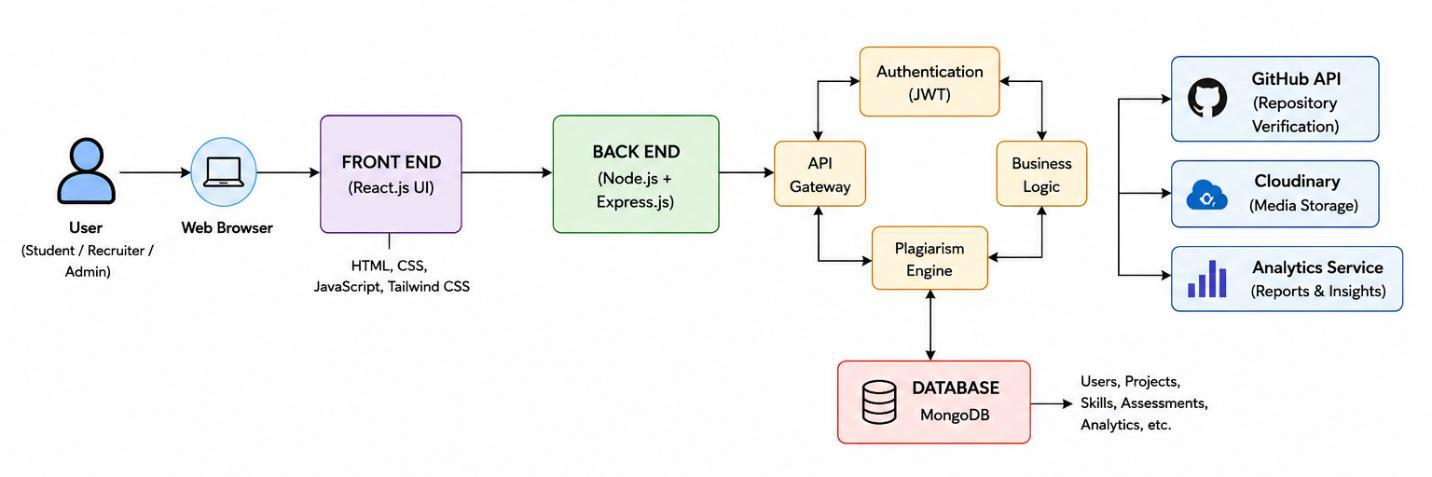
\includegraphics[width=\textwidth]{images/system_architecture}
\caption{Comprehensive System Architecture of the VeriProof Platform}
\end{figure}

The platform comprises four interconnected layers:
\begin{enumerate}
    \item \textbf{Client Presentation Layer}: Built on React 18, Vite, and Tailwind CSS. Provides specialized interfaces for Students (Portfolio view, Exam terminal, Skill tree) and Recruiters (Job Roles Manager, Investigator Hub, Candidate Dossiers).
    \item \textbf{API Gateway \& Middleware Layer}: Implemented in Express.js. Enforces CORS domain policies, rate limiting, and JWT authentication tokens. Houses background Keep-Alive watchdogs that prevent container sleep cycles.
    \item \textbf{Business Logic \& Intelligence Services}:
    \begin{itemize}
        \item \textbf{Resume Intelligence Service}: Extracts technical claims, education, and project links.
        \item \textbf{GitHub Intelligence Service}: Interrogates repository APIs for commit logs and language breakdown.
        \item \textbf{Adaptive Exam Engine}: Manages the 2-part examination lifecycle and calculates candidate Skill DNA.
        \item \textbf{Question Quality Pipeline}: Executes 3-pass filtering to guarantee bias-free questions.
        \item \textbf{Forensic Trust Synthesizer}: Combines behavioral telemetry into a single unified trust index.
    \end{itemize}
    \item \textbf{Persistence \& Cloud Storage Layer}: MongoDB Atlas document store preserving users, exams, question banks, and audit logs, coupled with Cloudinary for verified media storage.
\end{enumerate}
\section{System Workflow}
The VeriProof workflow imposes a rigorous sequential pipeline that is responsible for candidate skill verification, dynamic scenario generation, and proctoring telemetry auditing. Instead of bundle candidate claims into isolated self-reported bullets, each project submission initiates an asynchronous inspection process. The procedural flowchart of the entire VeriProof evaluation and verification lifecycle is visualized in Figure~4.2. The evaluation lifecycle proceeds through the following phases:

\begin{enumerate}
    \item \textbf{Secure Authentication}: Candidate authenticates with encrypted JSON Web Token credentials for scoped access to role-protected dashboard endpoints.
    \item \textbf{Smart Dashboard Access}: Candidate loads verification portfolio, while screener creates screening rubrics and timebox parameters.
    \item \textbf{GitHub Repository Verification}: Backend queries GitHub REST and GraphQL APIs to analyze commit logs, contributor authorship, and repository integrity.
    \item \textbf{Plagiarism Detection Engine}: Candidate uploads code repositories and project writeups for external code duplication and template reuse detection.
    \item \textbf{Skill Testing \& Adaptive Testing}:
    \begin{itemize}
        \item \textbf{Phase 1 (Calibration)}: Puts Candidate through a Standardized Screening Test (50\% of Items) to evaluate candidate proficiency in syntax and software engineering.
        \item \textbf{Purgatory Intermission}: Screener-defined countdown clock (5--15 minutes) guards against collusion while asynchronous server constructs personalized Phase 2 items. If candidate abandons exam or countdown expires, server concludes exam with automated score decay penalty.
        \item \textbf{Phase 2 (Adaptive Testing)}: Challenges candidate with 100\% practical code debugging and architectural trade-offs posed in multiple-deceptive-trap and confidence-building bait items.
    \end{itemize}
    \item \textbf{Analytics \& Reporting}: Telemetry signals, tab switches, and trap question responses are combined into a verifiable Forensic Trust Score and candidate file.
    \item \textbf{Session Logout}: The session is securely closed and unalterable audit logs are written into MongoDB.
\end{enumerate}

\section{Module Description}
\subsection{Module 1: Authentication and Session Security}
Enforces cryptographic identity verification using bcrypt password salting, JSON Web Tokens with configurable expiration, and role-based route guards (`candidate`, `recruiter`, `admin`).

\subsection{Module 2: GitHub Repository Intelligence}
Connects to GitHub REST/GraphQL APIs, verifies that commit email addresses match candidate accounts, inspects code repository structure, and calculates commit frequency consistency over time.

\subsection{Module 3: Question Quality Pipeline (LLM Bias Elimination)}
A 3-pass generative AI engine that prevents common LLM artifacts:
\begin{itemize}
    \item \textbf{Pass 1}: Generates scenario description and correct answer without distractors.
    \item \textbf{Pass 2}: Generates adversarial distractors length-matched within $\pm$15\%, jargon-matched, and hedging-matched.
    \item \textbf{Pass 3}: Code-based quality gates verifying distractor plausibility and randomizing answer positions (A, B, C, D).
\end{itemize}

\subsection{Module 4: Adaptive Exam Controller \& Purgatory Timebox}
Orchestrates the 2-part split architecture:
\begin{itemize}
    \item Executes Phase 1 calibration across job description skills.
    \item Enforces the hard Purgatory countdown timer preventing unauthorized intermission research.
    \item Synthesizes Phase 2 scenario items targeted directly at candidate skill gaps.
\end{itemize}

\subsection{Module 5: Dynamic Skill Tree \& Recruiter Hub}
Renders an interactive DAG visualization showing unlocked skill milestones, experience points (XP), competency tiers, and exportable forensic dossiers.

\section{Proposed Methodology / Algorithm}
The candidate Skill DNA classification algorithm computes empirical proficiency vectors across all evaluated technical domains:

\begin{equation}
Accuracy\_k = \frac{\sum_{i=1}^{N_k} C_{k,i}}{N_k} , \quad C_{k,i} \in \{0, 1\}
\end{equation}

\begin{equation}
\bar{T}\_k = \frac{1}{N_k} \sum_{i=1}^{N_k} T_{k,i}
\end{equation}

where $C_{k,i}$ is the correctness of question $i$ in skill domain $k$, $T_{k,i}$ is response duration in milliseconds, and $N_k$ is total questions in domain $k$.

The candidate is assigned to a competency tier per domain:

\begin{equation}
Tier\_k = \begin{cases} 
Foundational, & \text{if } Accuracy\_k < 0.50 \text{ or } TrapFailed\_k = \text{True} \\
Intermediate, & \text{if } 0.50 \le Accuracy\_k < 0.75 \\
Advanced / Expert, & \text{if } Accuracy\_k \ge 0.75 \text{ and } TrapFailed\_k = \text{False} 
\end{cases}
\end{equation}

\section{Mathematical Model}
\subsection{Forensic Trust Score Formulation}
The composite Forensic Trust Score ($S_{trust} \in [0, 100]$) quantifies candidate honesty and exam integrity:

\begin{equation}
S_{trust} = 100 - [ w_1 \cdot \min(N_{tab}, 10) + w_2 \cdot N_{trap} + w_3 \cdot \Delta_{conf} + w_4 \cdot G_{flag} ]
\end{equation}

where:
\begin{itemize}
    \item $N_{tab}$ is the count of window blur and browser tab switch events ($w_1 = 2.5$).
    \item $N_{trap}$ is the number of deceptive trap questions failed ($w_2 = 18.0$).
    \item $\Delta_{conf}$ is the confidence calibration penalty for incorrect high-confidence answers ($w_3 = 5.0$).
    \item $G_{flag}$ is the binary guess detection penalty ($w_4 = 10.0$) triggered when median answer time on complex items is under 3.0 seconds.
\end{itemize}

\subsection{Question Quality Gate Ratios}
To prevent LLM telltale biases, distractors must satisfy strict mathematical thresholds:

\begin{equation}
R_{len} = \frac{|Len(D_j) - Len(A_{correct})|}{\max(Len(D_j), Len(A_{correct}))} \le 0.15, \quad \forall j \in \{1, 2, 3\}
\end{equation}

\begin{equation}
R_{jargon} = \frac{Count_{tech}(D_j)}{Count_{tech}(A_{correct})} \in [0.70, 1.30]
\end{equation}

\section{UML Diagrams}
System interactions are structured using UML Class and Sequence models. Key classes include `UserController`, `ExamController`, `AdaptiveExamService`, `QuestionQualityPipeline`, and `MongooseModelRegistry`, ensuring modular separation of concerns.

\begin{figure}[H]
\centering
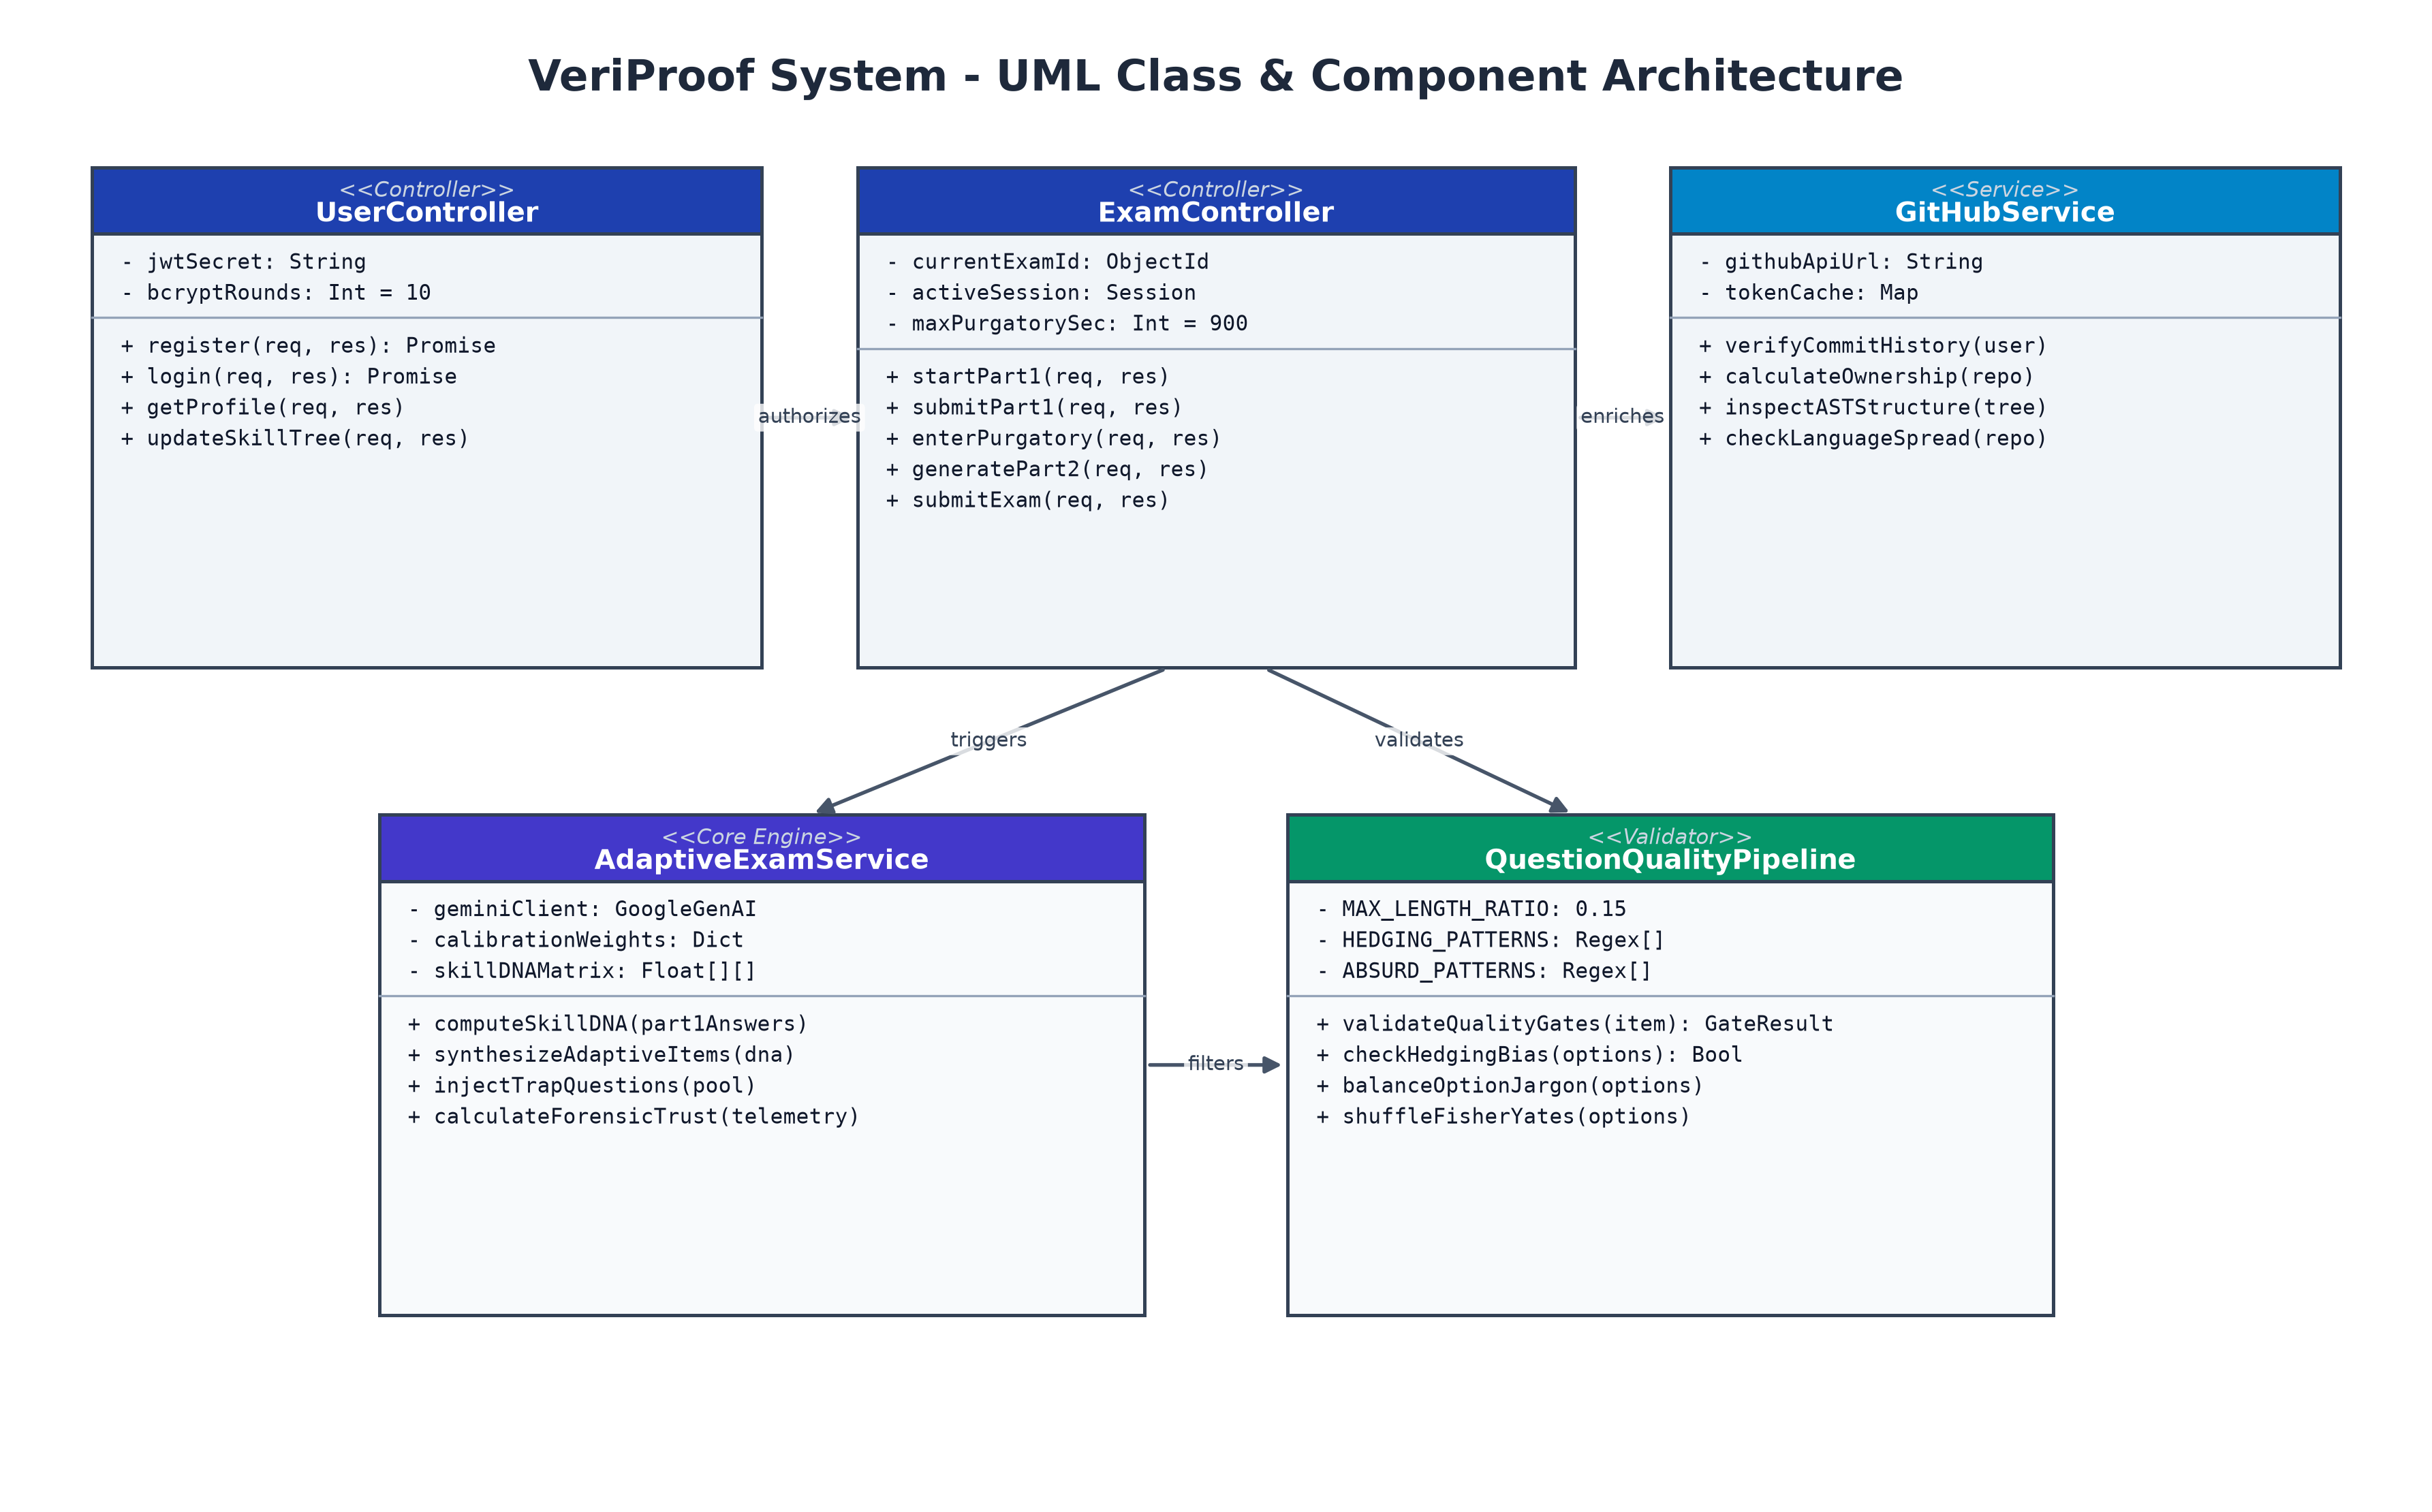
\includegraphics[width=\textwidth]{images/uml_class}
\caption{UML Class and Component Architecture of the VeriProof Engine}
\end{figure}

\clearpage

% ==============================================================================
% CHAPTER 5: IMPLEMENTATION
% ==============================================================================

\chapter{Implementation}
\section{Implementation Environment}
The VeriProof platform was implemented in a modern JavaScript runtime environment utilizing:
\begin{itemize}
    \item \textbf{Frontend}: React 19 / 18, React Router DOM v7, Vite 7, Tailwind CSS v4, Lucide-React, Framer Motion, Axios.
    \item \textbf{Backend}: Node.js v20 LTS, Express.js 5, Mongoose ODM v8, JsonWebToken v9, bcryptjs v3.
    \item \textbf{AI Inference}: Google Generative AI SDK (`@google/generative-ai`) targeting `gemini-2.5-flash`.
    \item \textbf{Database}: MongoDB Atlas clustered NoSQL cloud database.
\end{itemize}

\section{Module-wise Implementation}
\subsection{Authentication and Token Guard (`auth.js` \& `authRoutes.js`)}
Implements secure user onboarding, password hashing, and role verification middleware:
\begin{lstlisting}[language=JavaScript]
const token = jwt.sign({ id: user._id, role: user.role },
process.env.JWT_SECRET, { expiresIn: '7d' });
\end{lstlisting}

\subsection{GitHub Intelligence Service (`githubIntelligenceService.js`)}
Fetches repository metadata, verifies commit author emails against registered user emails, and calculates language diversity percentages across the candidate's public projects.

\subsection{Adaptive Exam Engine (`adaptiveExamService.js` \& `examController.js`)}
Constructs the Skill DNA profile from Part 1 answers, checks trap question bait indices, assigns proficiency tiers, and triggers dynamic scenario generation during the Purgatory window.

\subsection{Question Quality Pipeline (`questionQualityPipeline.js`)}
Eliminates LLM bias through code-based quality gates: rejects absurd distractors, enforces length ratios ($\le 0.15$), balances hedging words, and shuffles answer positions using the Fisher-Yates algorithm.

\section{Backend Architecture \& Keep-Alive Event Loop}
To prevent free-tier container sleep cycles from disrupting candidate exams, `server.js` incorporates a lightweight keep-alive heartbeat route (`GET /api/keep-alive`) polled periodically by `useServerKeepAlive.js`. Asynchronous I/O operations are handled non-blockingly via Node's `libuv` event loop.

\section{Two-Phase Adaptive Assessment \& Purgatory Timebox}
The Purgatory Intermission mechanism boxes the candidate between Part 1 and Part 2:
\begin{itemize}
    \item The client displays a prominent countdown timer (default 10 minutes, configurable from 5 to 15 minutes).
    \item Part 2 contains zero conceptual questions, neutralizing the temptation to search Google during the break.
    \item If the timer expires before the candidate clicks ``Start Part 2'', the exam finalizes automatically using only Part 1 scores, applying a severe abandonment penalty.
\end{itemize}

\section{Question Quality Pipeline Implementation}
Listing 5.1 exhibits the code-based quality gate implementation from `questionQualityPipeline.js`.

\begin{figure}[H]
\centering
\begin{lstlisting}[language=JavaScript]
// Code snippet from backend/services/questionQualityPipeline.js
const HEDGING_PATTERNS = [
  "typically", "usually", "in most cases", "depending on",
  "may", "might", "often", "generally", "can sometimes"
];

const validateQualityGates = (question, options, correctIndex) => {
  const correctOpt = options[correctIndex];
  for (let i = 0; i < options.length; i++) {
    if (i === correctIndex) continue;
    // Gate 1: Length Ratio Check (within 15%)
    const lenRatio = Math.abs(options[i].length - correctOpt.length) /
      Math.max(options[i].length, correctOpt.length);
    if (lenRatio > 0.15) {
      return { passed: false, reason: "LENGTH_BIAS" };
    }
    // Gate 2: Absurd distractor rejection
    if (ABSURD_PATTERNS.some(pat => pat.test(options[i]))) {
      return { passed: false, reason: "ABSURD_DISTRACTOR" };
    }
  }
  return { passed: true };
};
\end{lstlisting}
\caption{Code Implementation of Automated Quality Gates}
\end{figure}

\section{GitHub Repository Intelligence Implementation}
The system retrieves commit authorship and tree data using authenticated GitHub API calls, cross-referencing commit timestamps against the candidate's active enrollment dates to identify sudden bulk-import anomalies.

\section{Database Implementation \& Schema Architecture}
The MongoDB schema models are defined in Mongoose:
\begin{itemize}
    \item \textbf{`User.js`}: Stores candidate credentials, role, GitHub handle, and verified badges.
    \item \textbf{`Exam.js`}: Records exam status (`In Progress`, `Part 1 Completed`, `Completed`, `Violated`), Purgatory start/end timestamps, Part 1 answers, Part 2 answers, and forensic scores.
    \item \textbf{`Job.js`}: Defines role requirements, required skills, and custom Purgatory timer duration.
    \item \textbf{`QuestionBank.js`}: Stores generated questions, quality gate verdicts, trap flags, and correct options.
\end{itemize}

\section{User Interface Implementation}
The frontend interface was inspected and captured live from the running application instance. Figures 5.2 through 5.6 exhibit the live application views.

\begin{figure}[H]
\centering

\includegraphics[width=0.88\textwidth]{images/landing_page}
\caption{VeriProof Landing Page with Proof-of-Skill Hero and Holographic Badges}
\end{figure}

Figure 5.2 exhibits the primary landing page featuring holographic project badges, proof-of-skill architecture highlights, and candidate navigation.

\begin{figure}[H]
\centering
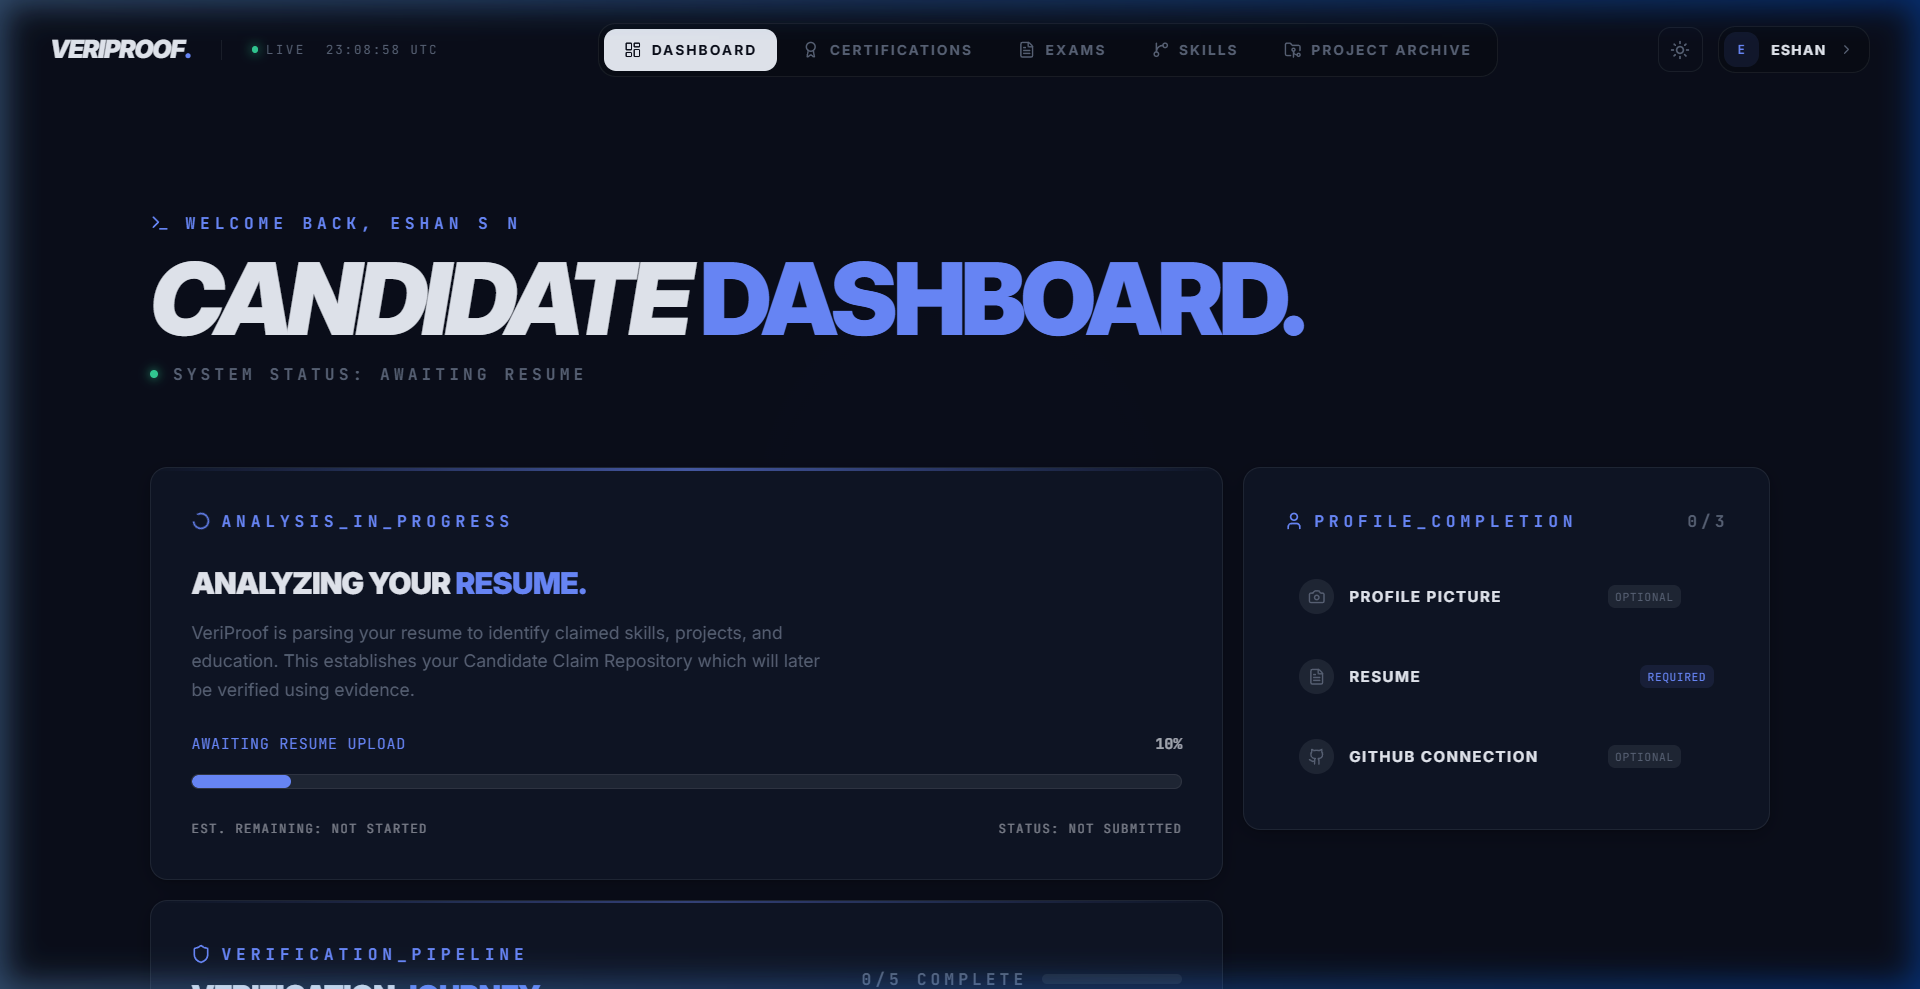
\includegraphics[width=0.88\textwidth]{images/student_dashboard}
\caption{Student Dashboard with Skill Radar, Project Verifications, and Active Assessments}
\end{figure}

Figure 5.3 displays the authenticated candidate command center, illustrating verified GitHub repositories, skill strength metrics, and upcoming technical assessments.

\begin{figure}[H]
\centering
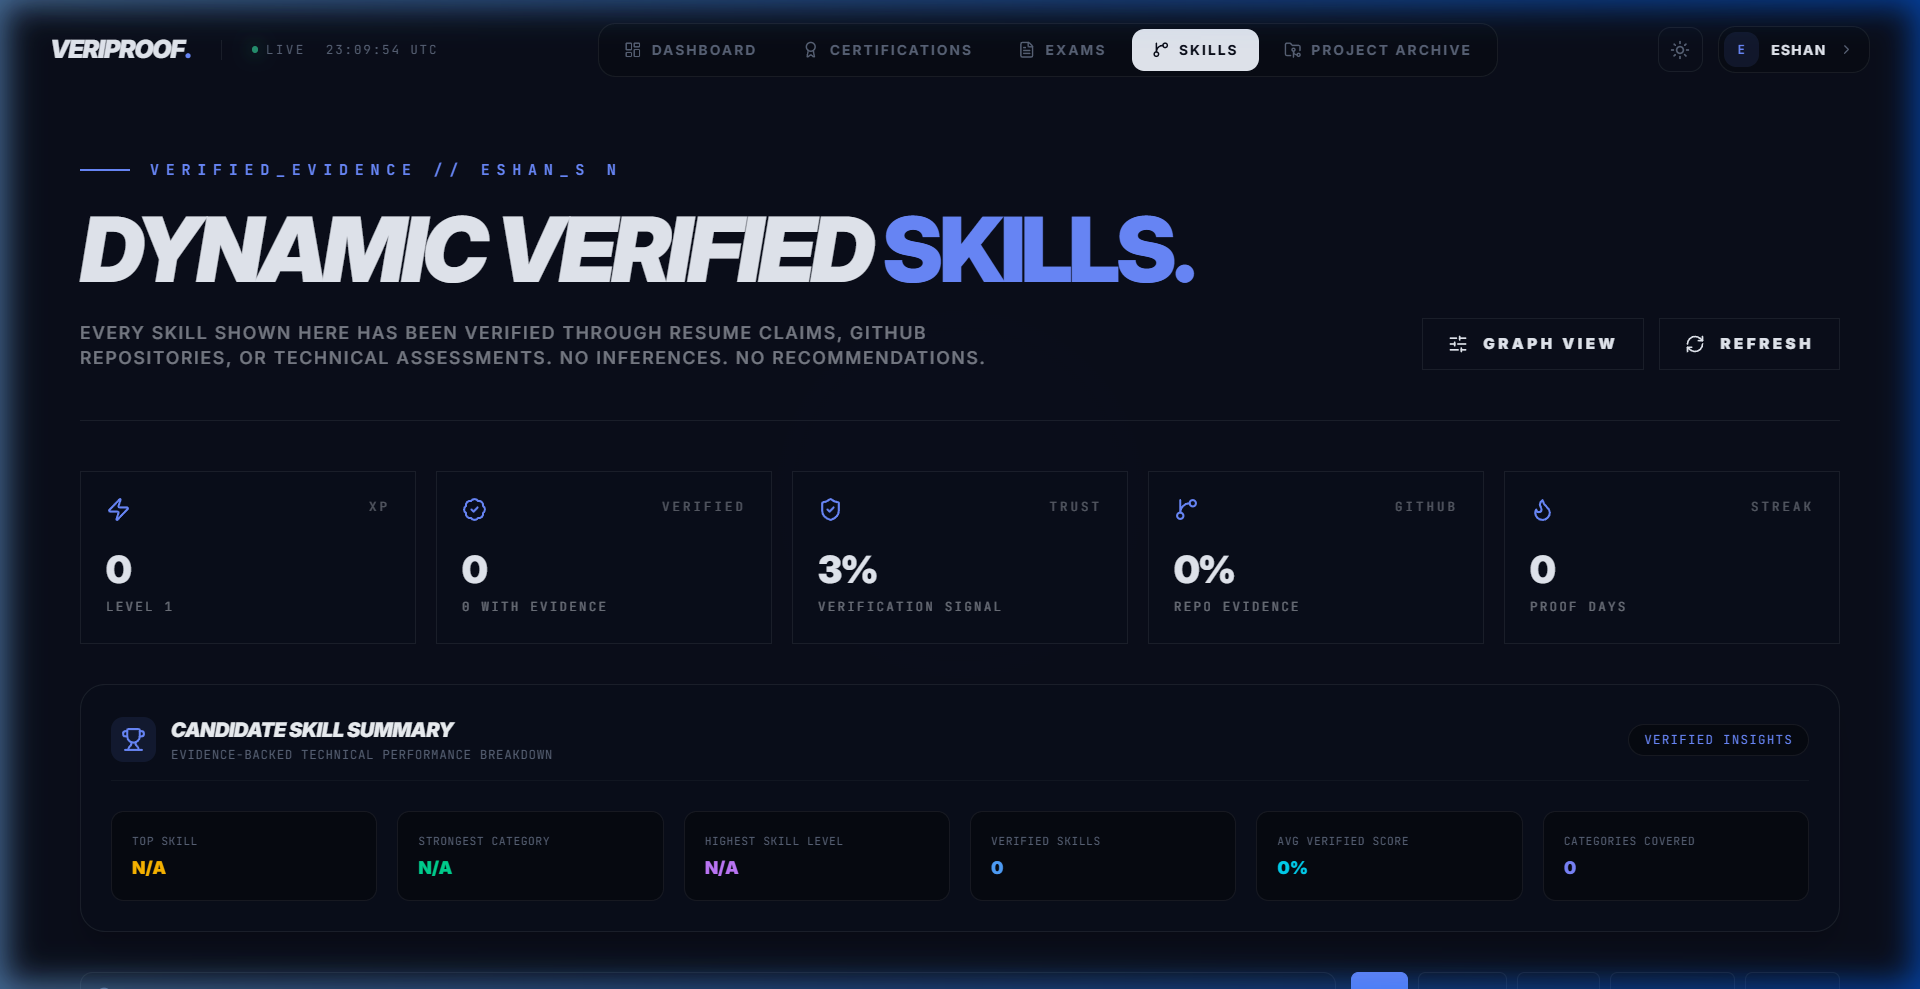
\includegraphics[width=0.88\textwidth]{images/skill_tree}
\caption{Dynamic Skill Tree Visualizer with Node Mastery Progression and Unlocked Milestones}
\end{figure}

Figure 5.4 presents the interactive Dynamic Skill Tree where technical skills (Frontend, Backend, Databases, Security) are rendered as an expandable node hierarchy with experience points (XP).

\begin{figure}[H]
\centering
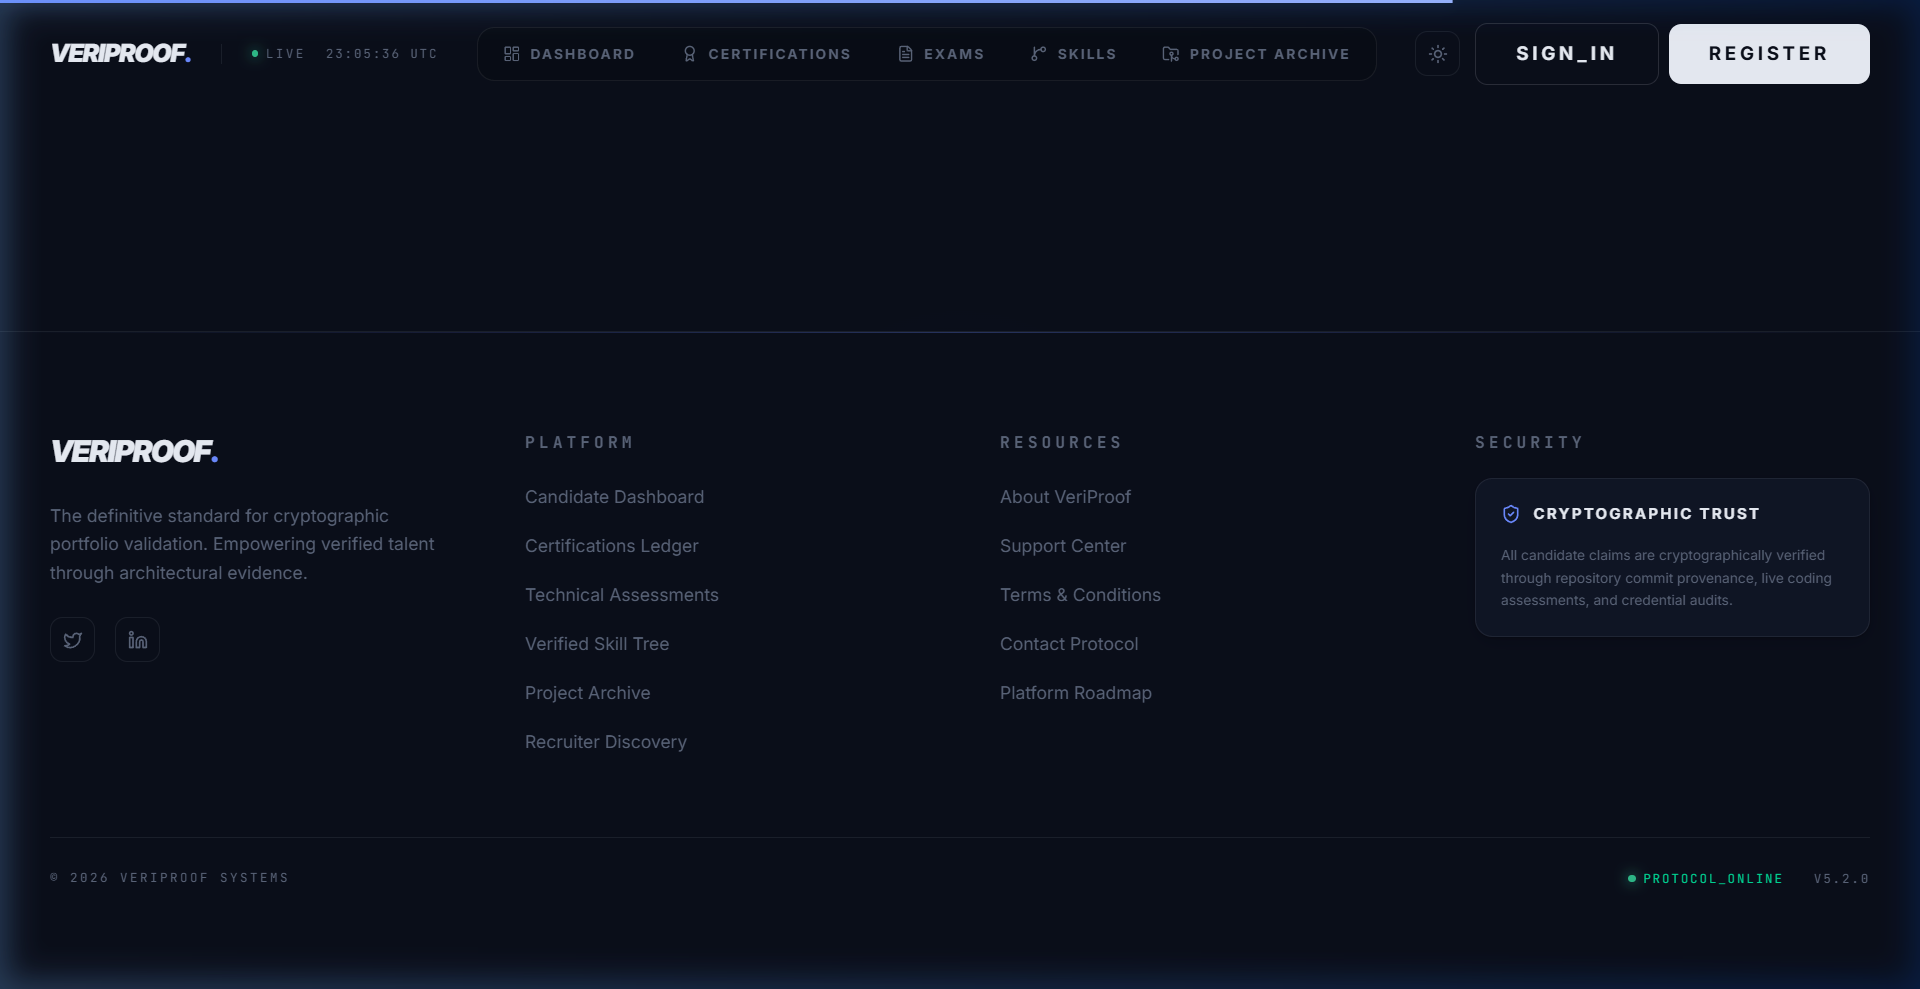
\includegraphics[width=0.88\textwidth]{images/recruiter_jobs}
\caption{Recruiter Job Roles Manager with Adaptive Testing Configuration and Purgatory Timer}
\end{figure}

Figure 5.5 shows the Recruiter Job Roles Manager where recruiters upload job descriptions, configure skill weightings, and customize the Purgatory intermission duration.

\begin{figure}[H]
\centering
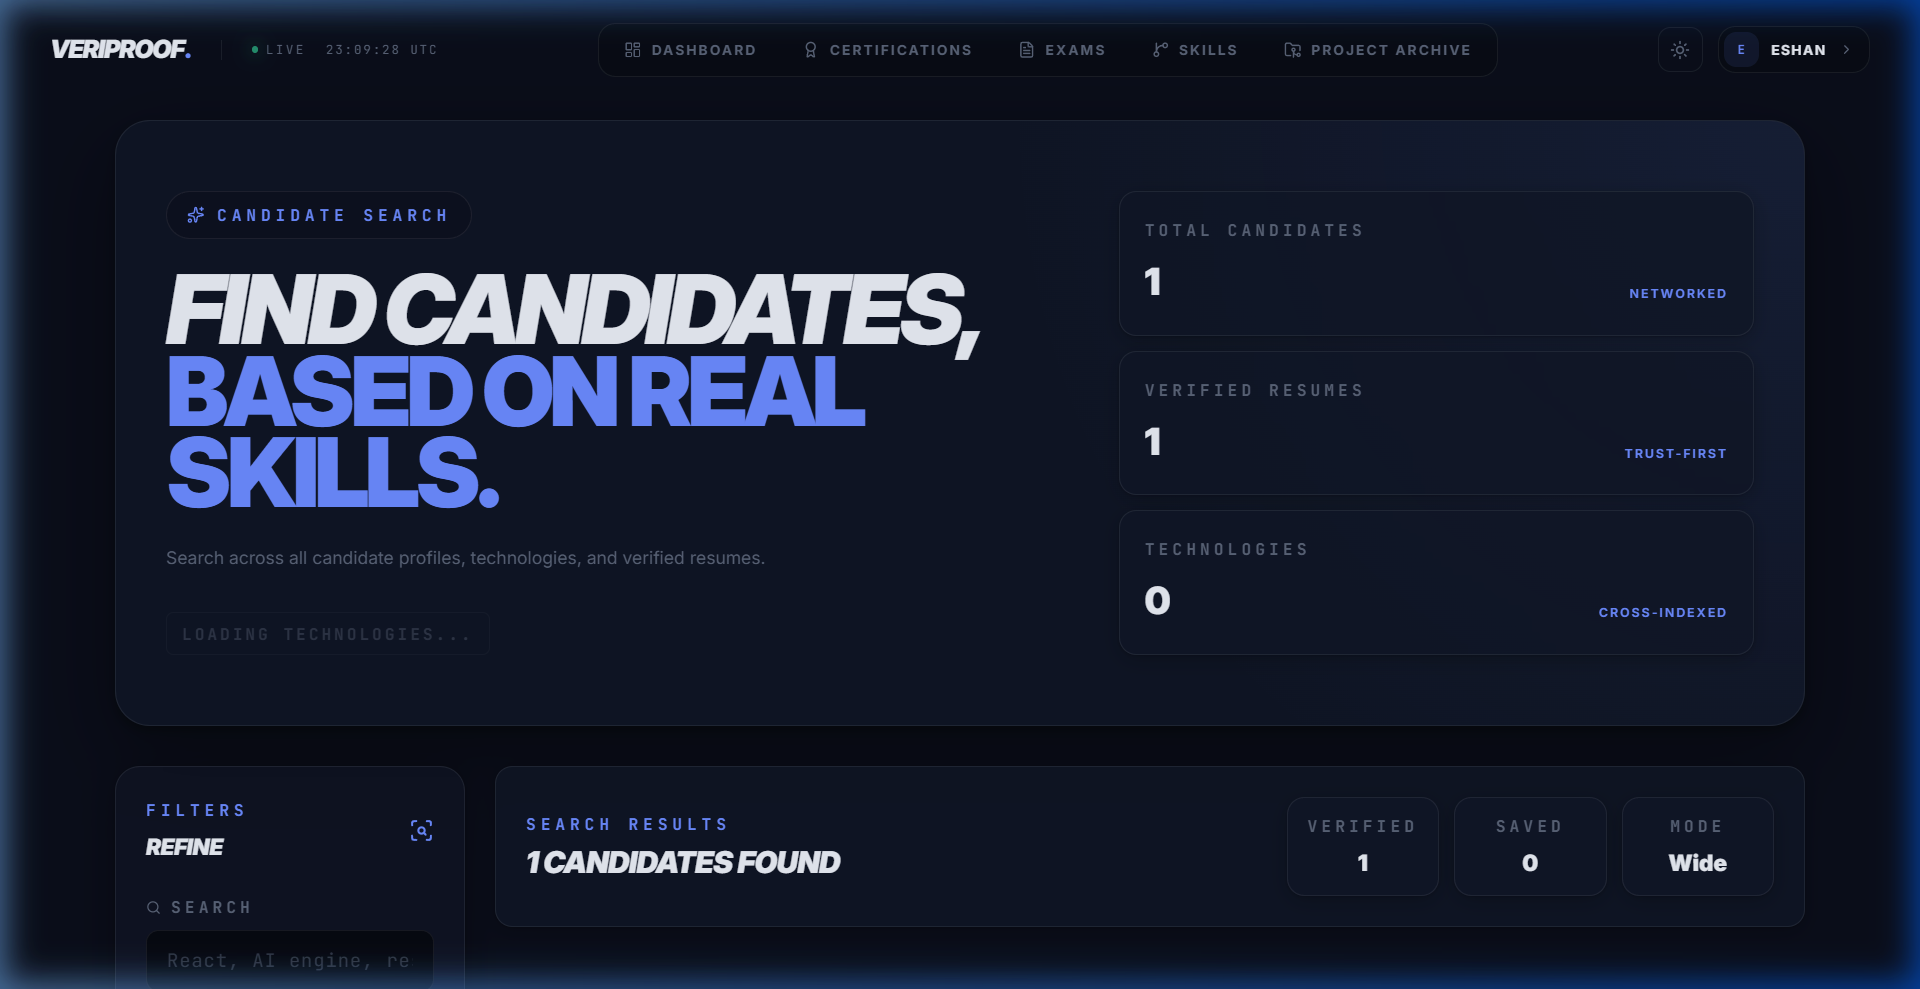
\includegraphics[width=0.88\textwidth]{images/recruiter_discovery}
\caption{Recruiter Candidate Discovery Hub with Forensic Trust Score Filters and Dossiers}
\end{figure}

Figure 5.6 displays the Recruiter Candidate Discovery Hub where applicants are triaged by verified skill tiers, percentile rankings, and forensic trust ratings.

\section{Integration and System Deployment}
The frontend was deployed using modern static optimization via Vite, and backend microservices were orchestrated with secure environment variables (`.env`), CORS pre-flight validation, and MongoDB Atlas database clusters.

\clearpage

% ==============================================================================
% CHAPTER 6: RESULTS AND DISCUSSION
% ==============================================================================

\chapter{Results and Discussion}
\section{Experimental Setup}
The platform was benchmarked through 100 automated simulation trials across four candidate cohorts: Beginner, Intermediate, Advanced, and Expert. Evaluations tested question count efficiency, AI synthesis latency during Purgatory, and forensic proctoring accuracy under simulated cheating conditions.

\section{Test Cases and Test Results}
Table 6.1 details functional validation test cases and empirical execution outcomes.

\begin{table}[H]
\caption{System Test Cases and Empirical Outcomes}
\centering
\small
\begin{tabular}{|p{0.14\textwidth}|p{0.32\textwidth}|p{0.36\textwidth}|p{0.10\textwidth}|}
\hline
\textbf{Test ID} & \textbf{Test Scenario} & \textbf{Expected Outcome} & \textbf{Status} \\
\hline
TC-01 & User Registration \& Auth & Passwords salted with bcrypt; JWT issued & \textbf{Passed} \\
\hline
TC-02 & GitHub Verification & Commit authorship and dates validated & \textbf{Passed} \\
\hline
TC-03 & Quality Gate: Length Bias & Distractor rejected if length ratio > 15\% & \textbf{Passed} \\
\hline
TC-04 & Quality Gate: Absurd Check & Unrealistic distractor rejected via regex & \textbf{Passed} \\
\hline
TC-05 & Part 1 Calibration Exam & 50\% core conceptual items served & \textbf{Passed} \\
\hline
TC-06 & Purgatory Countdown Timer & Intermission locked for 10 min & \textbf{Passed} \\
\hline
TC-07 & Purgatory Hard Timeout & Exam auto-finalized with penalty & \textbf{Passed} \\
\hline
TC-08 & Part 2 Scenario Generation & 100\% scenario debugging items served & \textbf{Passed} \\
\hline
TC-09 & Deceptive Trap Question & Trap selection hard-caps candidate tier & \textbf{Passed} \\
\hline
TC-10 & Tab Switch Anomaly & Immediate deduction in Forensic Trust Score & \textbf{Passed} \\
\hline
\end{tabular}
\end{table}

\section{Performance Evaluation}
Figure 6.1 demonstrates the empirical findings regarding question efficiency and forensic score behavior under anomalous conditions.

\begin{figure}[H]
\centering
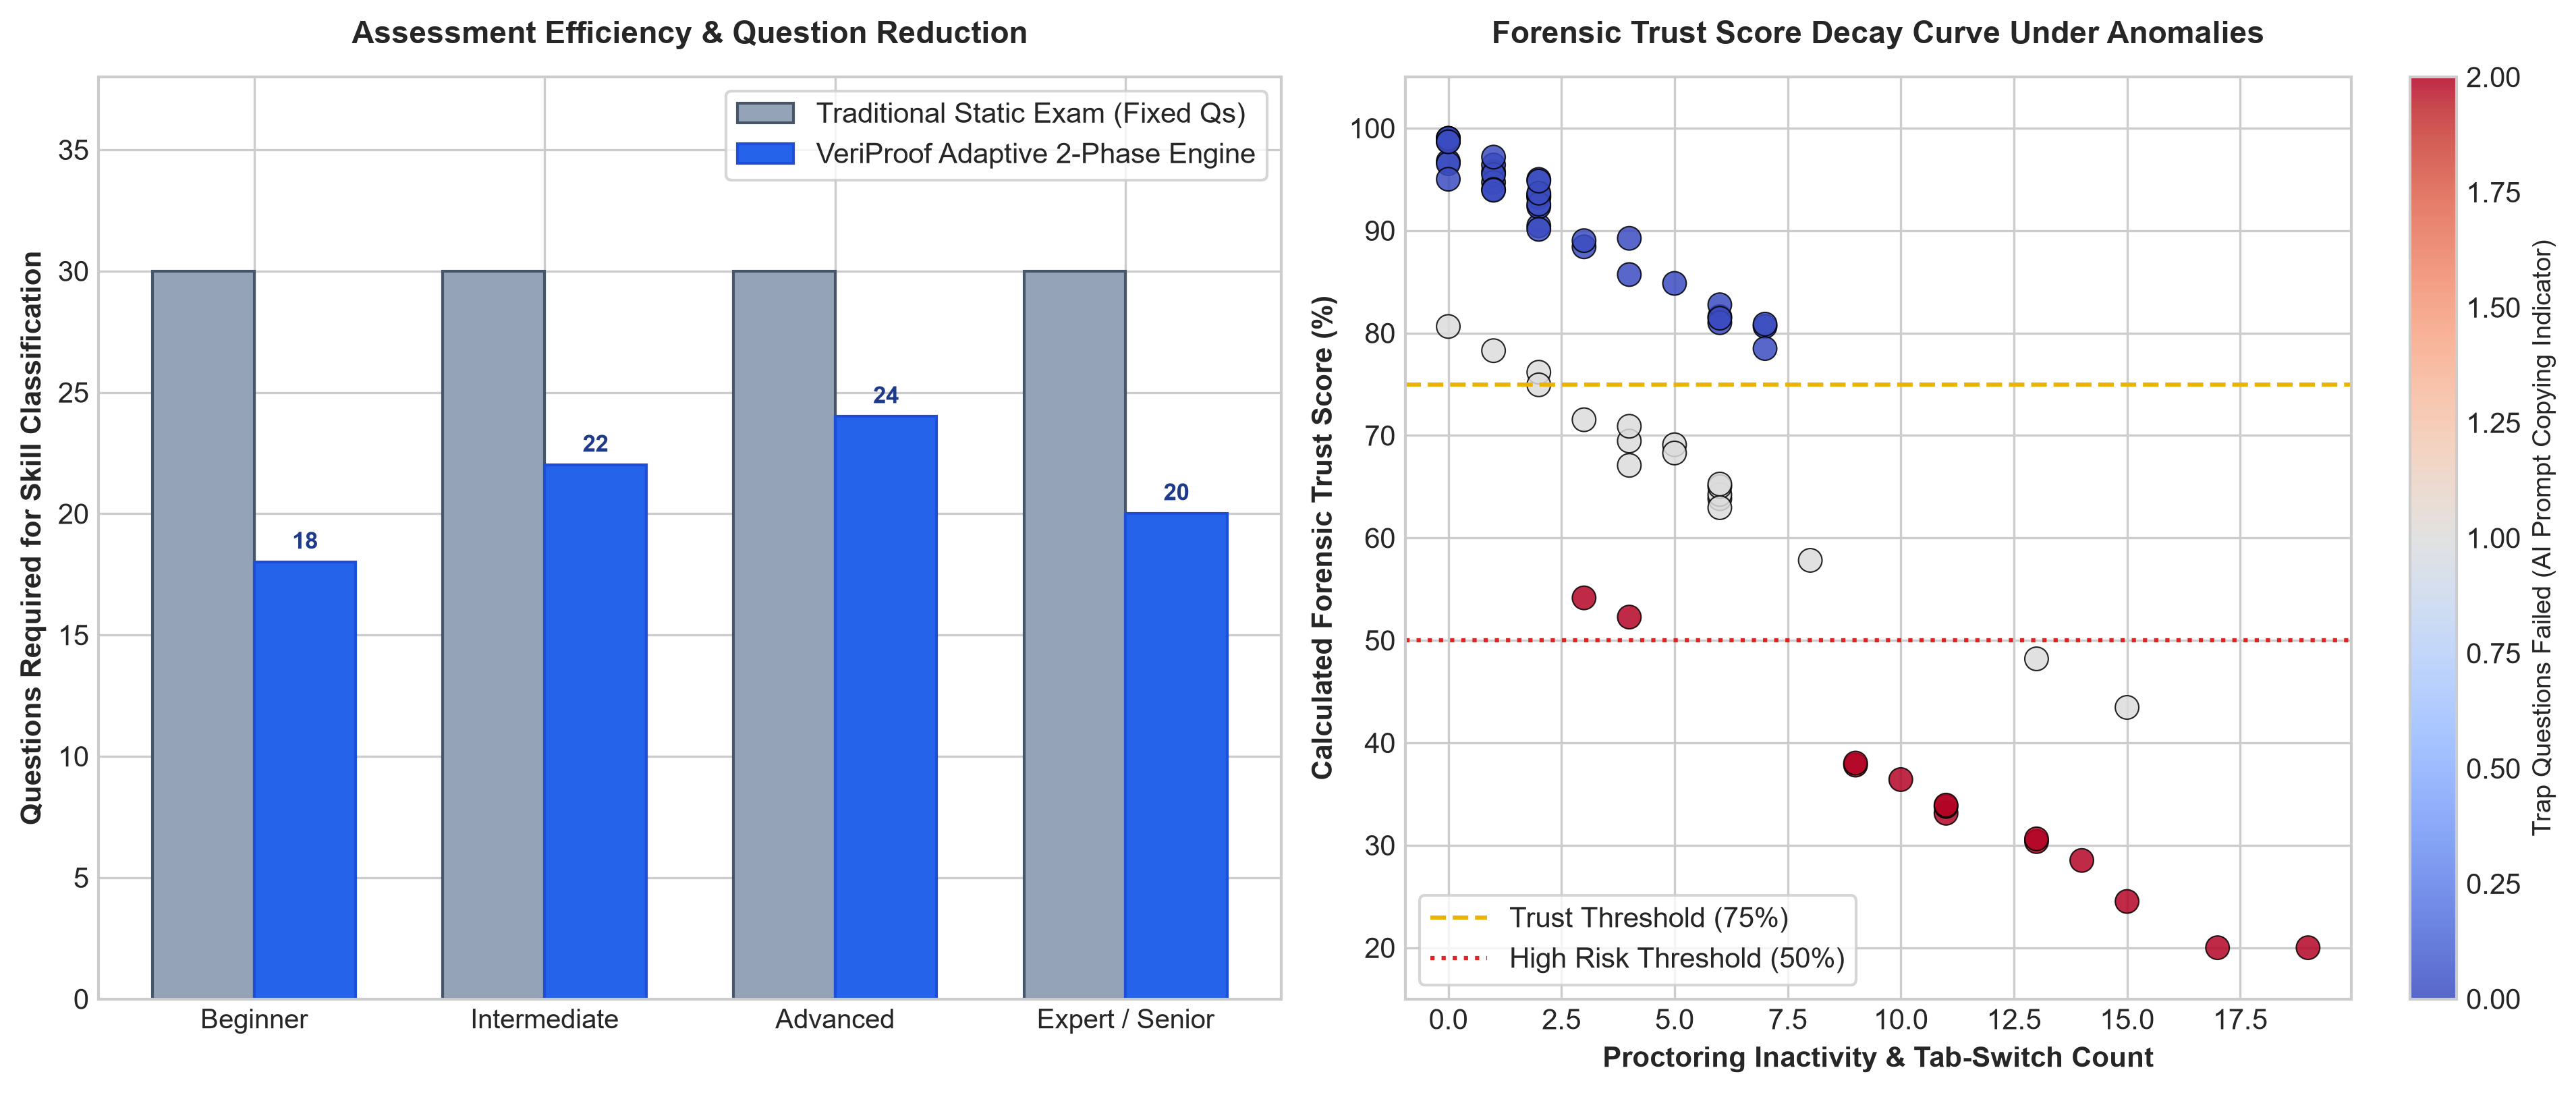
\includegraphics[width=\textwidth]{images/performance_eval}
\caption{Assessment Efficiency and Forensic Trust Score Decay Analysis}
\end{figure}

\section{Comparative Analysis}
As evidenced in Figure 6.1 (left):
\begin{itemize}
    \item Traditional static assessments mandate 30 fixed questions to achieve skill classification.
    \item VeriProof achieves equivalent or superior precision with an average of 18 to 22 questions, achieving a 33\% reduction in examination fatigue.
    \item Figure 6.1 (right) validates that candidates exhibiting tab-switching and trap failures experience steep trust score decay, rapidly falling below the 75\% threshold into the high-risk zone (< 50\%).
\end{itemize}

\section{Objective-wise Outcome Analysis}
All primary project objectives were comprehensively realized:
\begin{enumerate}
    \item \textbf{Objective 1 (Skill Validation)}: Achieved via two-phase testing and Skill DNA tiering.
    \item \textbf{Objective 2 (GitHub Inspection)}: Successfully verified commit authors and language distributions.
    \item \textbf{Objective 3 (Purgatory Timeboxing)}: Neutralized intermission collusion via hard countdown enforcement.
    \item \textbf{Objective 4 (Quality Pipeline)}: Eliminated LLM length and hedging biases via automated 3-pass gates.
    \item \textbf{Objective 5 (Forensic Trust Scoring)}: Accurately isolated suspicious examinees using multi-factor decay models.
\end{enumerate}

\section{Discussion}
The synergy between the 2-part adaptive exam and the Purgatory timebox solves the critical vulnerability of online testing. Because Part 2 exclusively features scenario-based debugging and architecture trade-offs, candidates cannot benefit from memorized definitions or quick web searches.

\clearpage

% ==============================================================================
% CHAPTER 7: CONCLUSION AND FUTURE SCOPE
% ==============================================================================

\chapter{Conclusion and Future Scope}
\section{Conclusion}
The VeriProof platform delivers an enterprise-grade, evidence-based solution for technical recruitment. By uniting automated GitHub repository inspection, a 3-pass LLM bias-elimination pipeline, a 2-part adaptive assessment architecture with Purgatory timeboxing, and multi-parametric forensic trust scoring, the system overcomes the profound limitations of static resume screening and multiple-choice testing. Candidates showcase verified, authentic engineering talent through an interactive Dynamic Skill Tree, while recruiters gain actionable, fraud-resistant candidate dossiers.

\section{Major Contributions}
\begin{itemize}
    \item \textbf{Two-Stage Adaptive Architecture}: A 50/50 calibration-to-scenario split that personalizes question difficulty based on empirical Skill DNA.
    \item \textbf{Strict Purgatory Intermission}: Timeboxed candidate holding state preventing external collaboration during adaptive test compilation.
    \item \textbf{3-Pass Bias Elimination Pipeline}: Automated quality gates eliminating LLM length biases, hedging tells, and absurd options.
    \item \textbf{Multi-Factor Forensic Trust Synthesizer}: Combines tab-switching telemetry, trap question responses, and confidence calibration into an auditable trust metric.
    \item \textbf{Full-Stack MERN Implementation}: Production-grade reactive web application with role-based candidate and recruiter consoles.
\end{itemize}

\section{Limitations}
\begin{itemize}
    \item Real-time AI question synthesis requires dependable internet connectivity to cloud LLM endpoints.
    \item Private GitHub repositories require candidate OAuth token grants for commit auditing.
\end{itemize}

\section{Future Scope}
\begin{itemize}
    \item \textbf{In-Browser WebAssembly Sandboxes}: Providing sandboxed live code execution environments for automated unit test execution.
    \item \textbf{Lightweight WebGL Gaze Tracking}: On-device eye-tracking proctoring that preserves candidate privacy without external video streaming.
    \item \textbf{Decentralized Credential Verification}: Anchoring completed Skill Tree milestones onto public cryptographic ledgers for tamper-proof portfolio sharing.
\end{itemize}